\documentclass[Main]{subfiles}
\begin{document}

\section{Deployment View}
Systemet er bygget op af en fjernbetjening, dronen, samt modtagerenheden på dronen, vist på Figur \ref{Fig:DeploymentViewOverview}.

\begin{figure}[H]
\centering
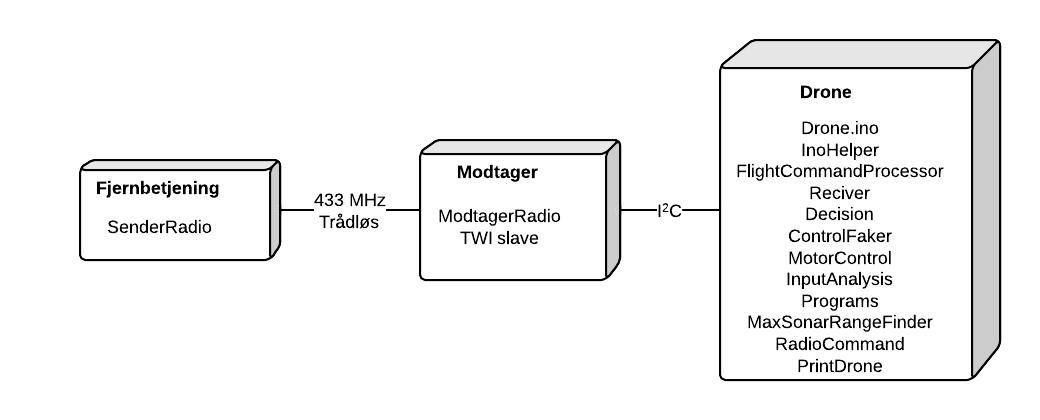
\includegraphics[width = 0.70 \textwidth]{DeploymentViewOverview}
\caption{Deployment View diagram}
\label{Fig:DeploymentViewOverview}
\end{figure}

Fjernbetjeningen sender sine signaler til dronen vha. det trådløse 433 MHz-signal, som opfanges af modtager-enheden.
Herefter sættes signalets værdi til rådighed, således dronen kan læse det igennem \itoc -forbindelsen.



\subsection{Protokoller}

\subsubsection{Fjernbetjening til modtager}

\begin{wrapfigure}{r}{0.5\textwidth}
  \centering
	\begin{tabular}{l l}
	\hline
	\textbf{Kommando} 	& \textbf{Indhold i bytes} \\ \hline
	Let 				& \code{0x3F} + \code{0b0000001x} \\
	Autoland 			& \code{0x3F} + \code{0b0000010x} \\
	Fremad 				& \code{0x3F} + \code{0b0000100x} \\
	Roter til højre 	& \code{0x3F} + \code{0b0000101x} \\
	Roter til venstre 	& \code{0x3F} + \code{0b0000110x} \\
	Roter til højre 	& \code{0x3F} + \code{0b0000111x} \\
	Stop 				& \code{0x3F} + \code{0b0001000x} \\
	Inkrementer højde 	& \code{0x3F} + \code{0b0001001x} \\
	Dekrementer højde 	& \code{0x3F} + \code{0b0001010x} \\ \hline	
  	\end{tabular}
  \makeatletter\def\@captype{table}\makeatother% "Change float to table"
  
\caption{Kommandoer sendt fra fjernbetjeningen}
\label{Tab:kommandoer}
\end{wrapfigure}

Ved tryk på knapperne på fjernbetjeningen sendes et signal til modtageren.
Signalet består af 2 bytes, hvoraf det første er en programindikator og den anden er selve programmet.

Desværre står det sidste bit og svinger, hvilket kan være ganske kritisk for, hvilket program der bliver kørt og af den årsag shift'es alle bit én plads op i den sidste byte før forsendelse og én bit ned ved modtagelse.
Dette giver mulighed for at sende $2^7 = 128$ programmer til eksekvering.

%Derudover kan det første byte indeholde forskellige indikatorer, hvilket giver mulighed for 256 forskellige typer beskeder, der hver indeholder 128 forskellige værdier.
Kommandoer der kan sendes vises i Tabel \ref{Tab:kommandoer}.



\subsubsection{Modtager til drone}
Når en pakke er modtaget, bliver den pakket ud og de to bytes ligges i en output buffer\fxnote{RBK -- forsætter her. Skriv også gerne noget om alt den sikkerhed der er i signalforbindelse.}




\end{document}